\documentclass[a4paper,12pt]{article}

\usepackage{times}
\usepackage{changepage}
\usepackage{setspace}
\usepackage{caption}
\usepackage{sidecap}
\usepackage{graphicx}
\usepackage[document]{ragged2e}
\usepackage{geometry}
 \geometry{
 top=35mm,
 }

\begin{document}
\pagenumbering{gobble}
\setlength{\parindent}{0em}
\doublespacing
\captionsetup{labelformat=empty}

\begin{center}
{\huge PACCMAN User/Developer Guide}

(Python Analysis of Conformal Cooling Molds And/or desigNs)
\end{center}

\bigskip

This guide is meant to be used as a resource for using, adding to, or integrating the PACCMAN program. 
It is expected that users will have a package manager such as Anaconda or another program with Numpy, Scipy, Matplotlib, etc.

\medskip

In order to install Pytest with Anaconda, open the Anaconda Powershell Prompt and run the command "conda install -c anaconda pytest ".

\medskip

Feedback is welcome. Please report all bugs to hughfeehan353 on Github. Thanks.

\section*{Basic Use:}

When run, the program first presents three options.
\begin{adjustwidth}{1cm}{}
Selecting "N" uses the first mold material properties (KM1, etc.) and then asks the user to choose the heat transfer coefficient correlation.

Selecting "M" compares the three mold materials using the Gnielinski correlation.

Selecting "H" compares the three heat transfer coefficient correlations using the first mold material property (KM1, etc.).
\end{adjustwidth}

\medskip

For all three choices, the program asks the user if they would like to save graphs of the average heat cycle temperature over time.
\begin{adjustwidth}{1cm}{}
Choosing "Y", downloads the graph in .png and .eps formats.

Choosing "N" will not download the graphs
\end{adjustwidth}
\clearpage

\medskip
\begin{center}
\begin{figure}
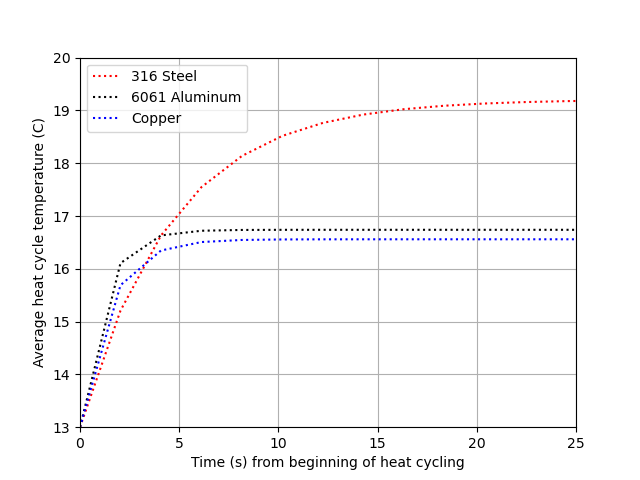
\includegraphics[width=\linewidth]{paccman-example-graph.png}
\caption{An example graph for option "M" (mold material comparison). }
\end{figure}
\end{center}

The program is written so that by changing the variables, it can analyize any desired conformal cooling design and will report the following data: 
\begin{adjustwidth}{1cm}{}

flow velocity, kinematic viscosity, Reynolds number, Prandl number, Farcy friction factor, heat transfer coefficient, average heat cycle temperature of the mold, time constant, and coolant pressure drop.
\end{adjustwidth}
\clearpage

\section*{Application Fundamentals for Advanced Use:}

At the beginning, the program initializes and assigns all the basic variables. These can all be changed, or the list can be added to in order to improve the function of the program. However, they are all necessary for the program to function properly so should not be completely omitted.

\medskip

Afterwards, all the necessary functions are defined. Similarly, these cannot be removed as they are necessary for the program’s function but could be added to.

\medskip

At this point there is an “if” statement to check for the user’s desired function for the program.  This “if” statement contains all of the program’s calculation functions in order to ensure that nothing will break if the user chooses an invalid letter.

\medskip

The first thing inside the “if” statement are some calculations that must be completed no matter the chosen choice of the program’s function. 

\medskip

The rest of the calculations contain nested “if” and “elif” statements so that the correct variables are used for the chosen program function.

\medskip

Once the calculations are completed, the program creates a plot of the average heat cycle temperature over time that the user has the choice of downloading.

\medskip

The program can be tested using Pytest by running the "pytest" command in the program's directory.

\end{document}